This section will cover which features were modified and added to AirSim to reach the desired behaviour. Each section will look at the challenges faced and discuss previous approaches. The sections will also explain which bits of existing code the feature is based off, or if the feature was written from scratch.

\subsection{Requirements}


\subsection{Multiple Entities}
The first modification to be made to the simulator was to make sure that it could handle multiple agents. This was an essential step as the simulator could not be used if having several agents at once was not possible. Currently, the simulator is primarily designed for one agent. After initial research, the simulator should have been able to handle two vehicles if this was added to the startup configuration. However, this did not work in Unity. 

The first step was to modify the existing APIs so that the vehicles could be accessed individually. To do this, all vehicles were added to a global list. Each vehicle was also given a unique identifying name. The next step was to add an argument to each API specifying the vehicle.  When a vehicle API was called, Unity would first iterate over the map looking for the corresponding vehicle. Once the entity was found Unity would then forward the API request to that vehicle. This change had to be made throughout AirSim tracing the call from the user interaction in Python to Unity. 

The main challenges faced when doing this was originally trying to adapt the configuration file. As this had not been properly implemented in Unity yet, time was spent trying to debug this issue. Eventually, it was discovered that adding the vehicles manually to the scene before starting would be easier. 

Currently, if two vehicles are given the same name the second vehicle will spawn, but the API calls will only be redirected to the first vehicle. This can easily be changed so that either both entities should behave in the same way, or that the second entity does not spawn. This behaviour however was seen as unimportant and have been left out for the time being. 
 

\subsection{Spawning Entities at Runtime}



% \begin{figure}[h]
%     \centering
%     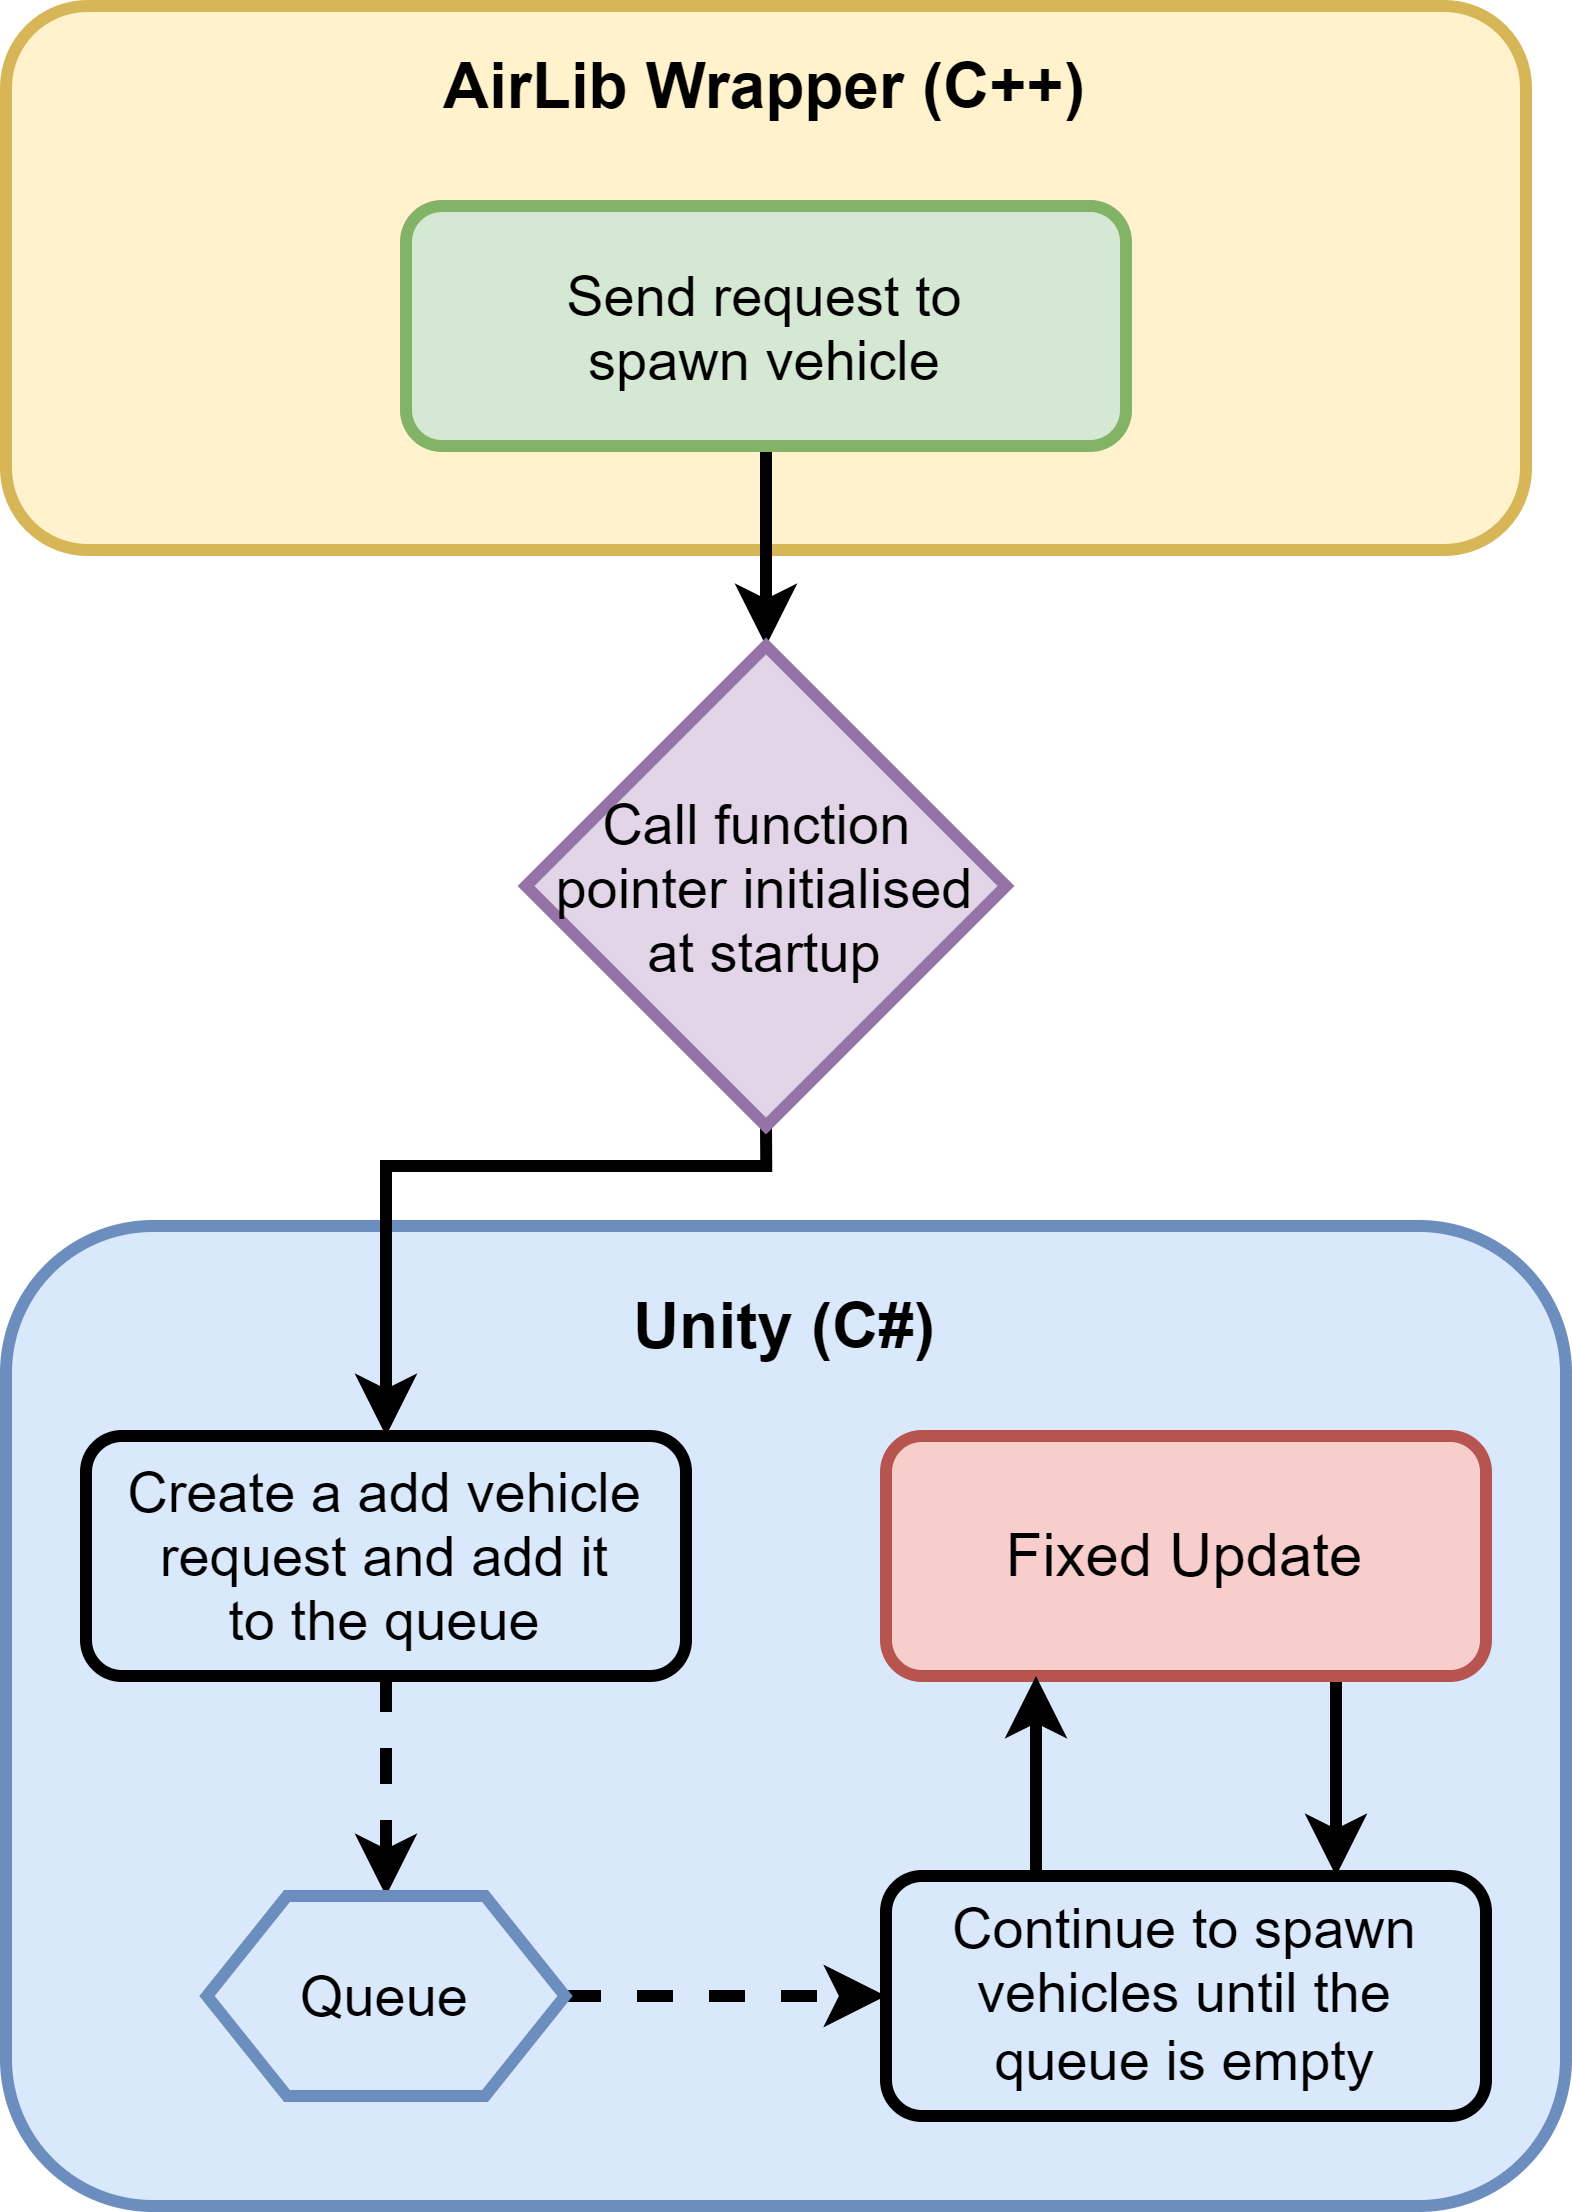
\includegraphics[width=0.5\textwidth]{06_Implementation/00_AirSim/Diagrams/spawnVehicle.png}
%     \caption{Unity is not thread-safe, so the server has to interact with the simulator through shared memory.} \label{06:spawnVehicle}
% \end{figure}


Being able to spawn entities at runtime was a desired feature as it would allow the users to have full control of the simulation through the APIs. This was not an existing feature as the simulator was not designed to simulate several entities at once. As mentioned in the section above, multiple vehicles could be declared in the configuration file. This file however is only loaded at the start and never reloaded whilst the simulator is running. 

\begin{wrapfigure}{r}{0.5\textwidth}
    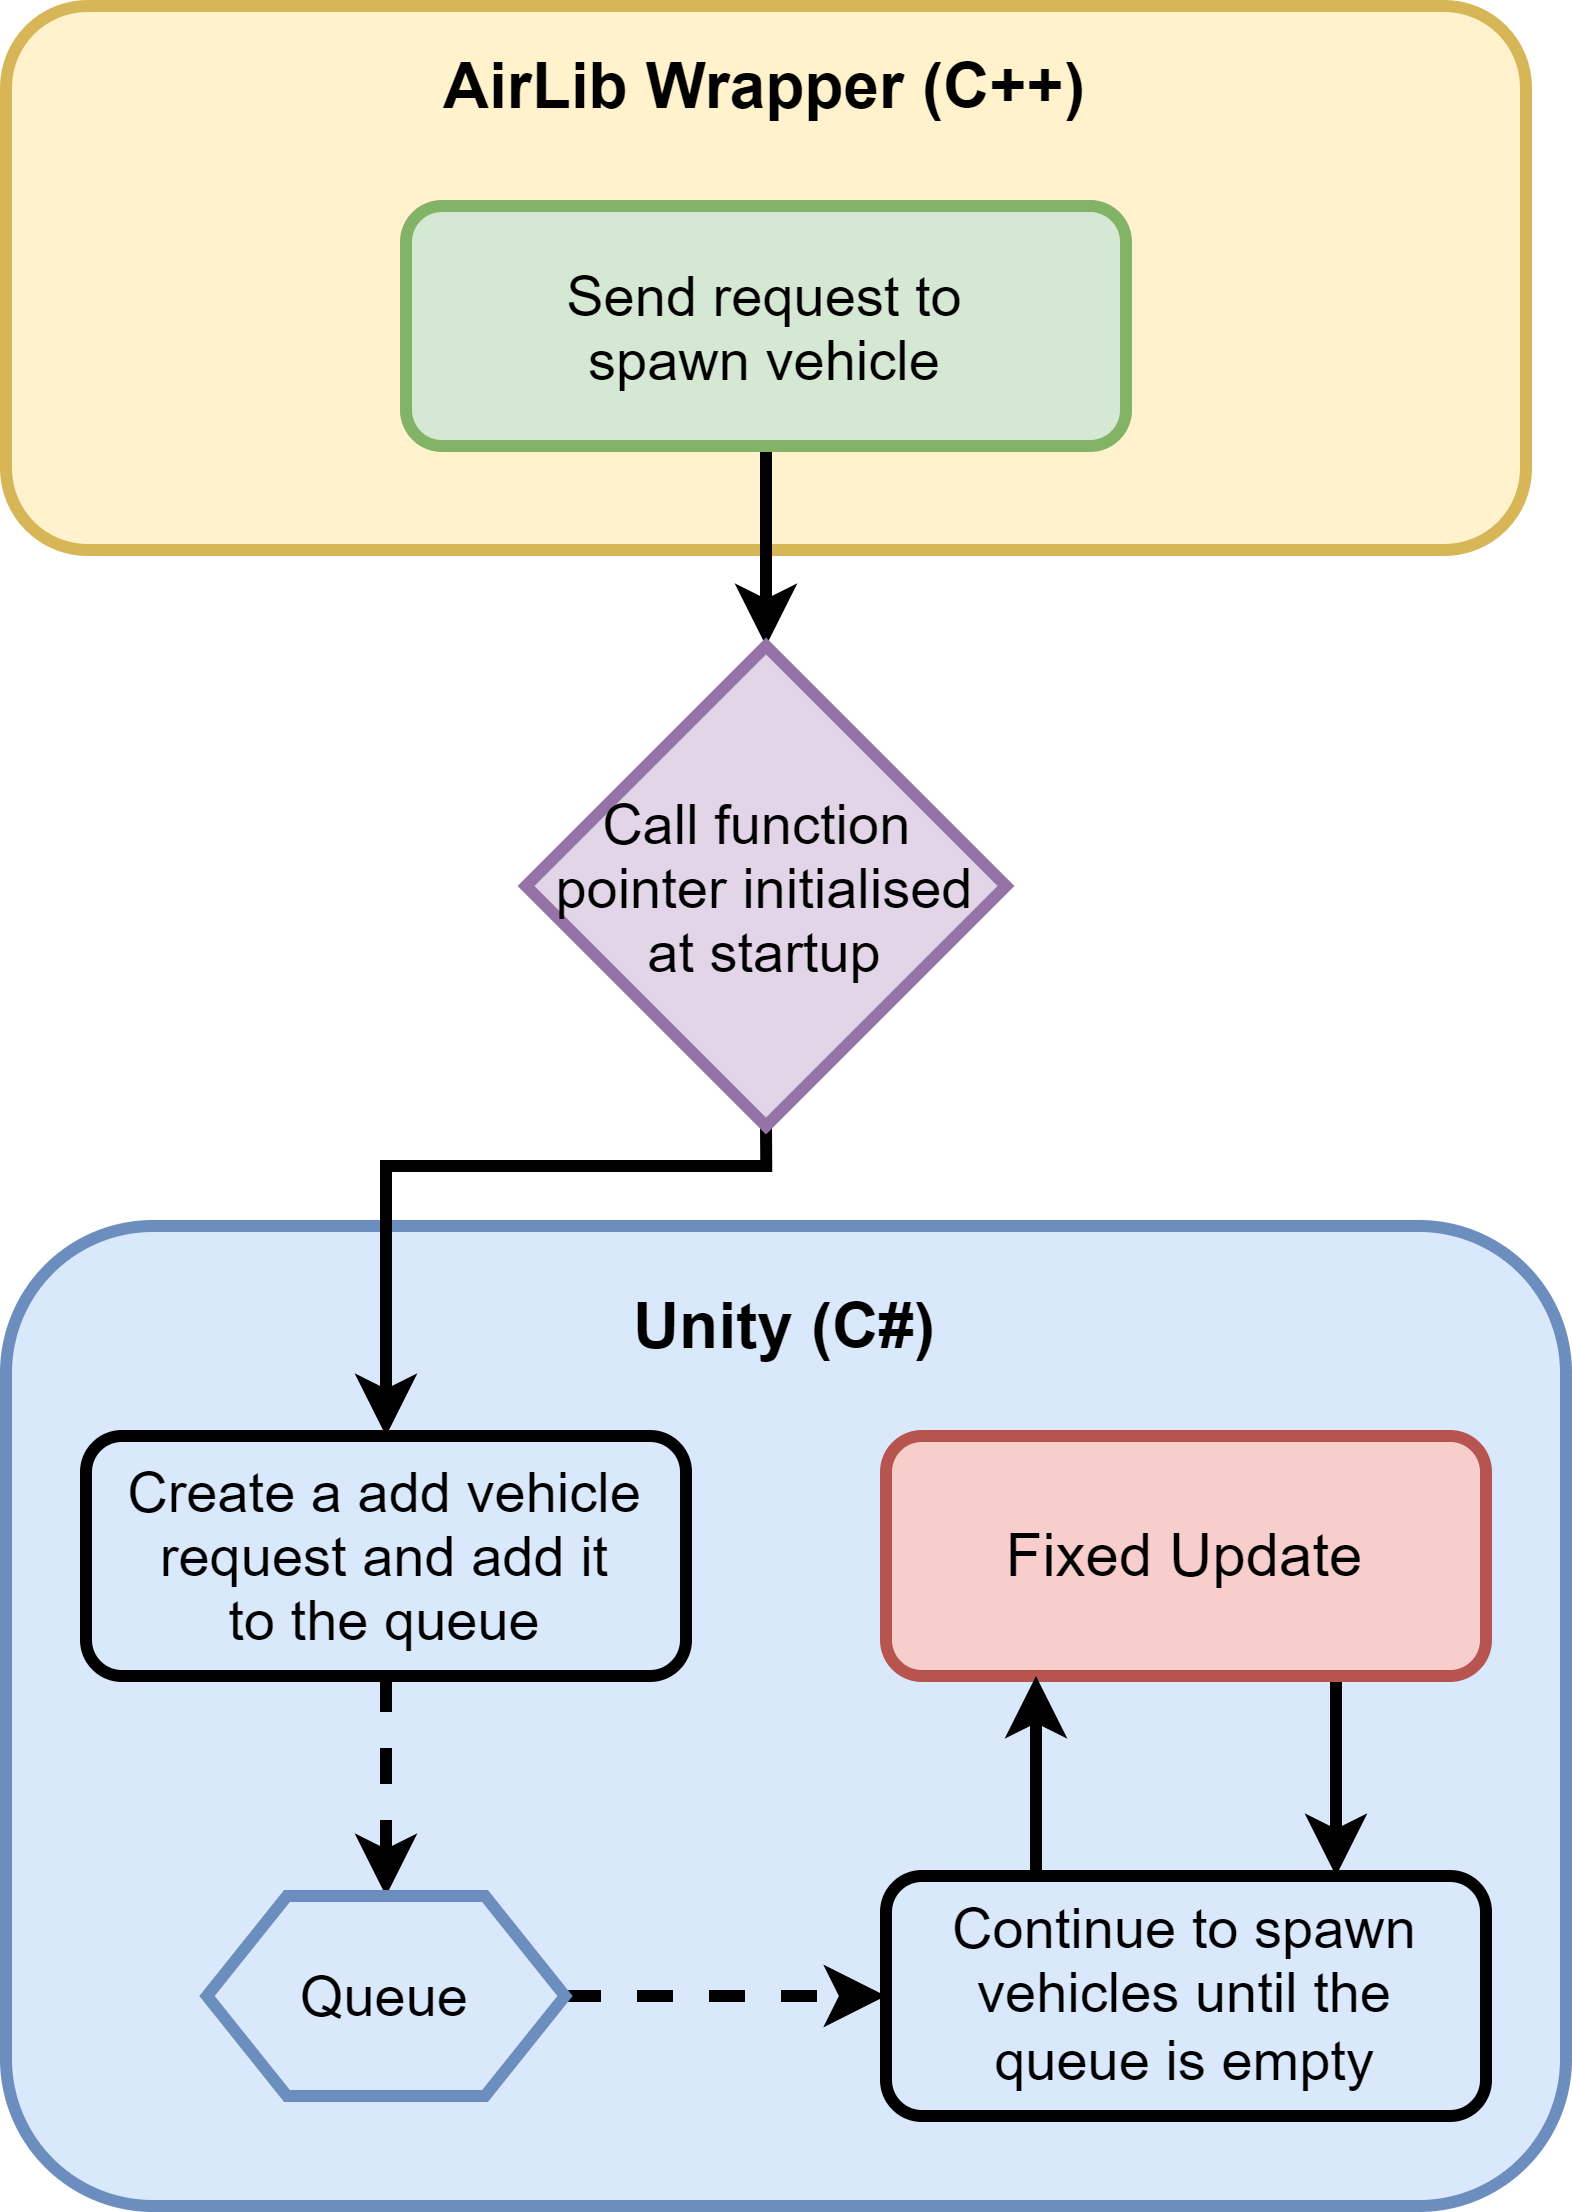
\includegraphics[width=0.5\textwidth]{06_Implementation/00_AirSim/Diagrams/spawnVehicle.png}
    \caption{Unity is not thread-safe, so the server has to interact with the simulator through shared memory. For simplicity, the figure ignores everything that happens before the wrapper.} \label{06:spawnVehicle}
\end{wrapfigure}

The first change that had to be made to AirSim was to add the new API. The API would take in four arguments: the vehicle type, the identifying name, the spawn coordinates and the initial rotation. The first issue that had to be resolved was that Unity is not thread-safe. This means that the server could not directly interact with the simulator behaviour. As can be observed from Figure~\ref{06:spawnVehicle}, this was resolved by creating a request which was added to a queue. The fixed update cycle would then check if this queue was empty on every game tick. This means that the user can quickly send several requests to the server and they all get spawned within a few game ticks of each other. 

Another change that had to be made was when the server was instantiated. In the original implementation, the server was connected to the vehicle itself. This meant that the server was only running when there was a vehicle in the scene. To fix this a server object was added to the game scene. The server would now open when the server started, and close when the simulator stopped. (See Figure~\ref{A:MonobehaviorFlow} in the Appendix). Moving the server to a separate game object caused a few issues with the action order. However, these were fixed by moving the vehicle initialisation to the awake stage. Pedestrians would use the same structure once added. 

The alternative to spawning the entities at runtime is to have an object pool, where all of the entities can wait until needed. However, this is not needed as the vehicles are fast to load. For more complex entities this could be a better option. The disadvantage of using this method is that there will then be a limit to the number of entities as users cannot generate more if they run out. 


\subsection{Video feed} \label{06:VideoFeed}
One of the requirements for this project was to have sensing APIs (Section~\ref{}). With the Unity game engine, AirSim can return a captured frame to the user interaction layer. The return is a struct that consists of the camera settings, image type, image width and height and the binary image data. This is then converted back into an image in Python. This API had to be updated as the frames rate returned by the server was low, especially when introducing more vehicles. 

\begin{figure}[p]
    \centering
    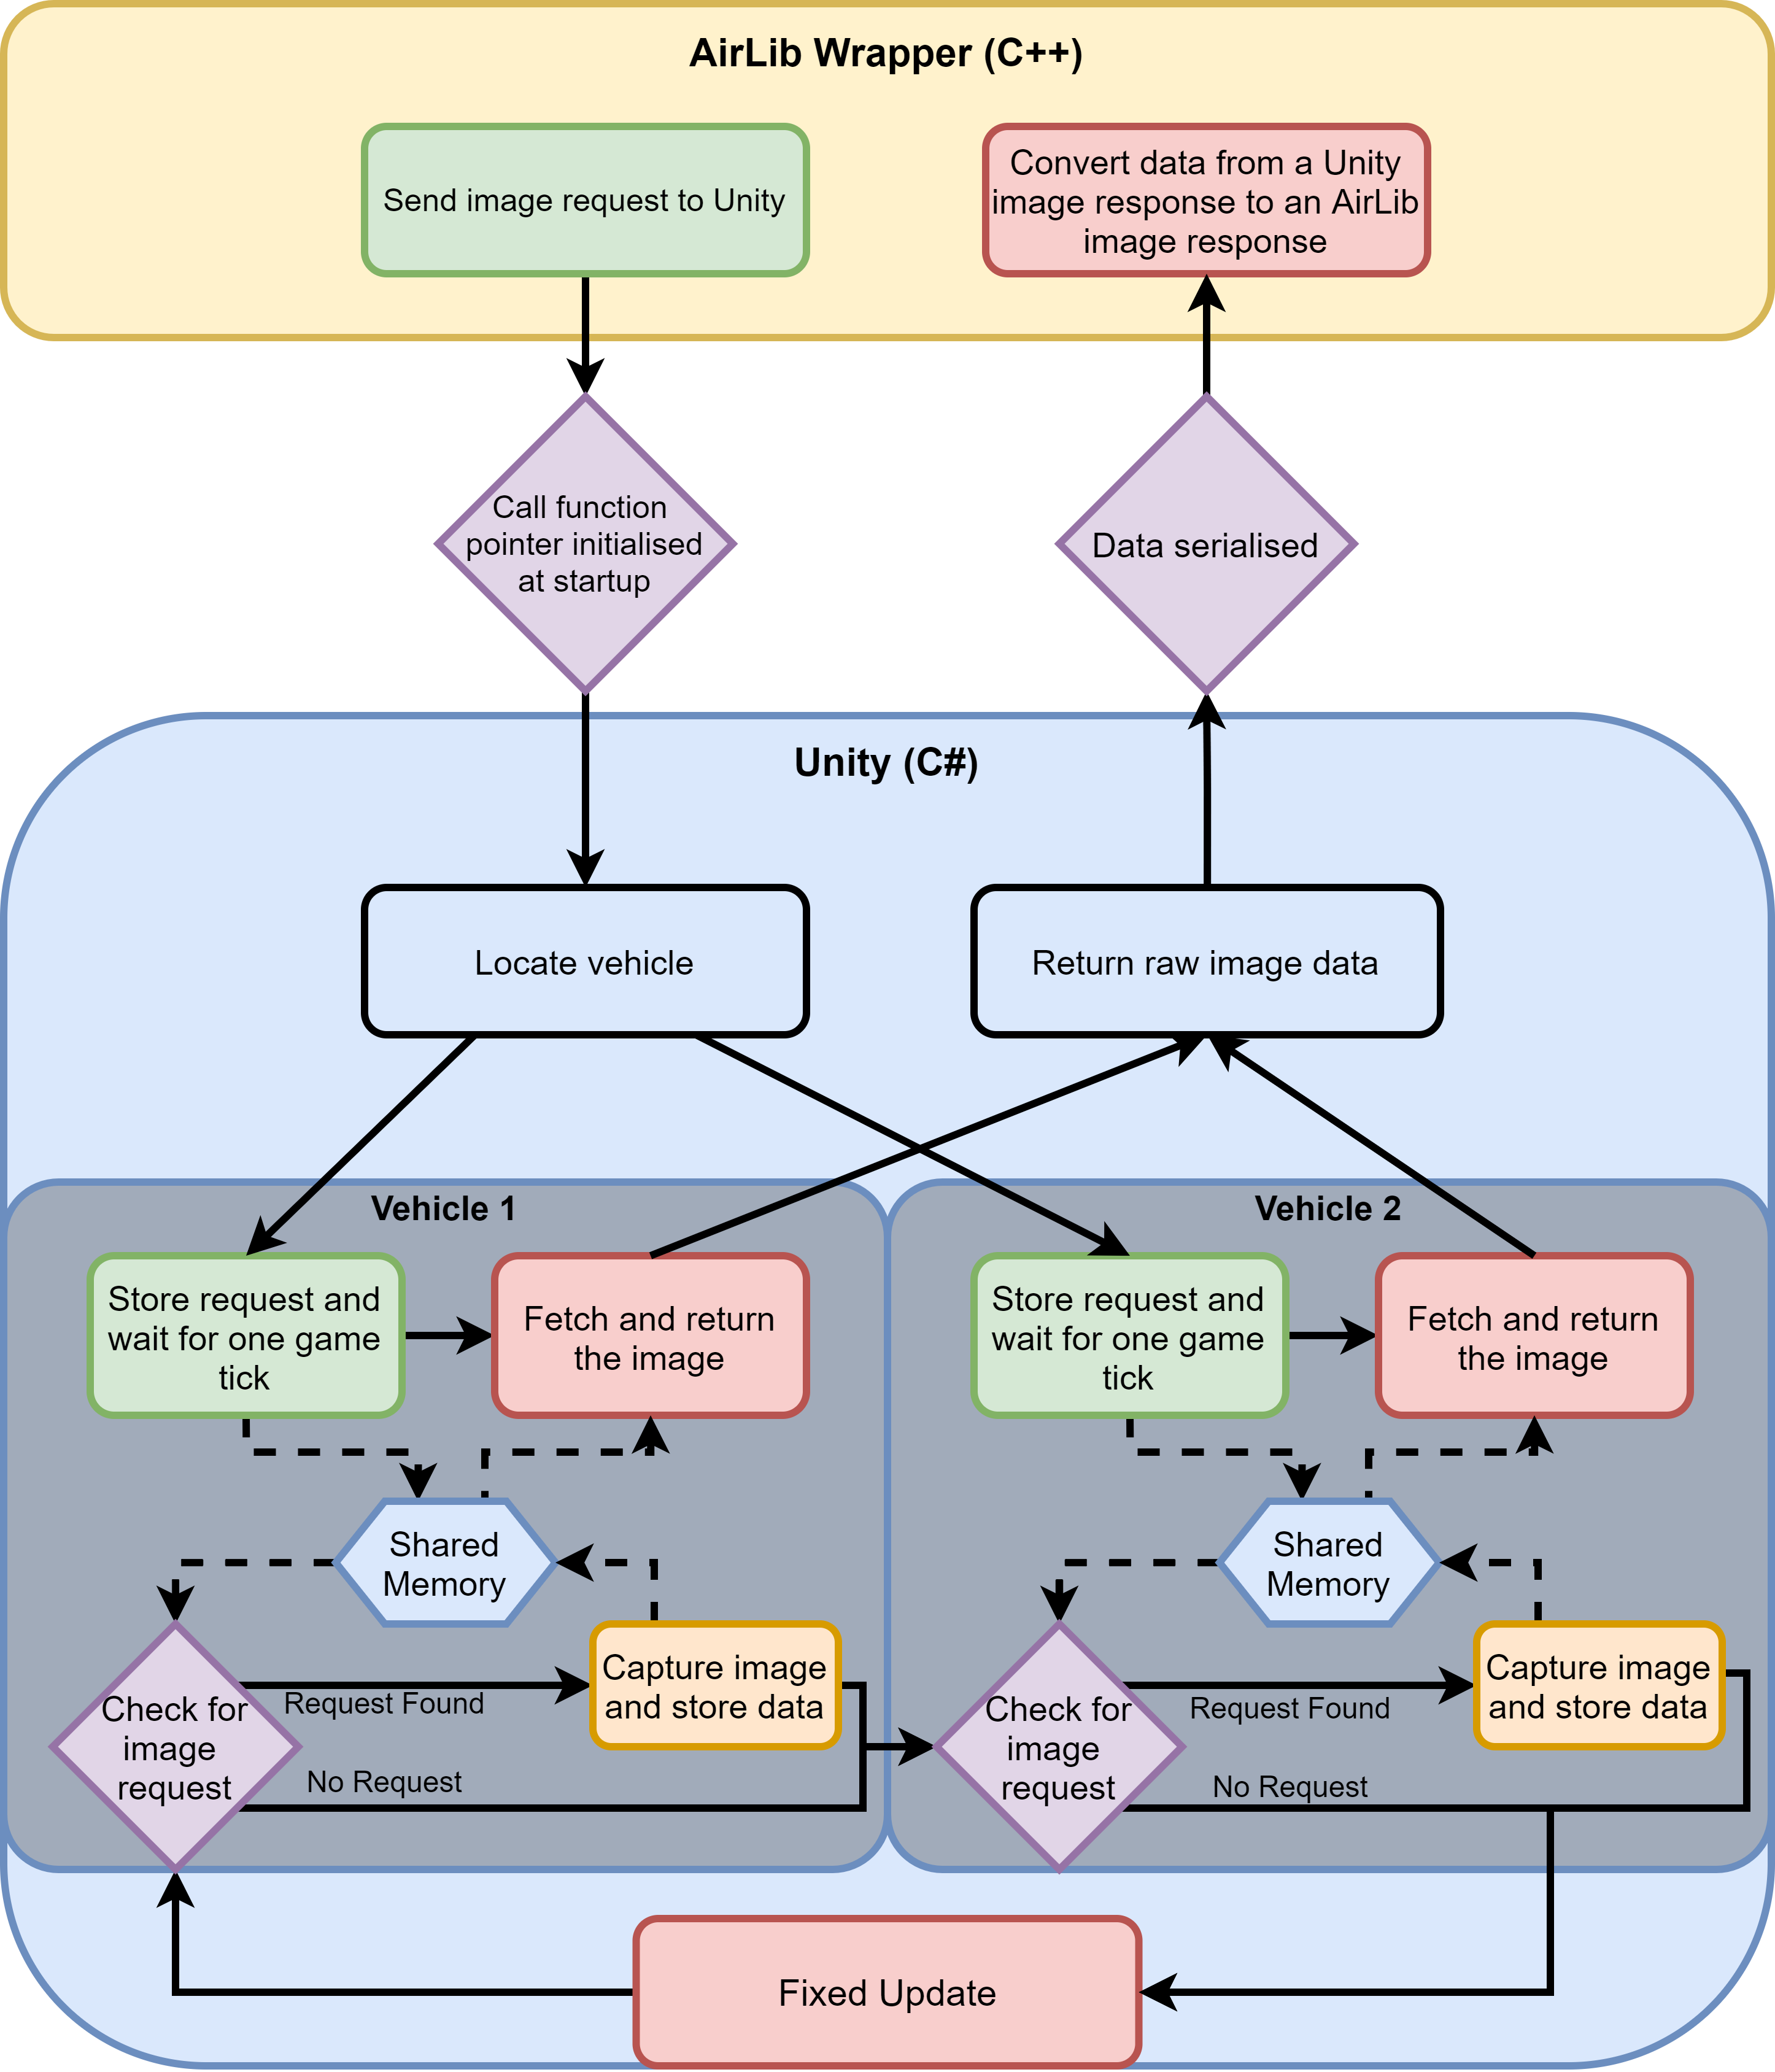
\includegraphics[width=1.0\textwidth]{06_Implementation/00_AirSim/Diagrams/imagecapture.png}
    \caption{} \label{06:imageCapture}
\end{figure}

Figure~\ref{06:imageCapture} shows the existing implementation of how the fetch image API works. Note, only the AirLib wrapper and Unity components are displayed in the diagram. The first part is to pass the image request to the correct vehicle. The image request contains the camera name and type. Unity supports different image types such as scene, which renders the textures as usual, depth and infrared. The call then waits for one game tick and then returns the image response. As can be seen, this method has little impact on the simulator performance as capturing one image does not take long. However, the issue arises when several image requests are happening at once. As the server is single-threaded, the first request has to return before the next one is processed. Using coroutines in Python does not resolve this issue either as the requests will just be queued. One option is to open several servers as mentioned in Subsection~\ref{05:dividingServer}. This however can produce a large overhead when there are many entities. The simulator is running at 120 game ticks per second.

Up to 5 cameras, this method works well. Assuming the calls happen one after the other and a capture takes one game tick, all 5 cameras can return an image in 5 ticks. This means that the frame rate is 24 frames per second. However, two vehicles would half that to 12 FPS, and so on. The output frame rate would therefore be $120/(n*c)$ where n is the number of vehicles and c is the number of cameras per vehicle. The advantage of this method is that it does not impact the tick rate of the simulator. 

\begin{wrapfigure}{r}{0.7\textwidth}
    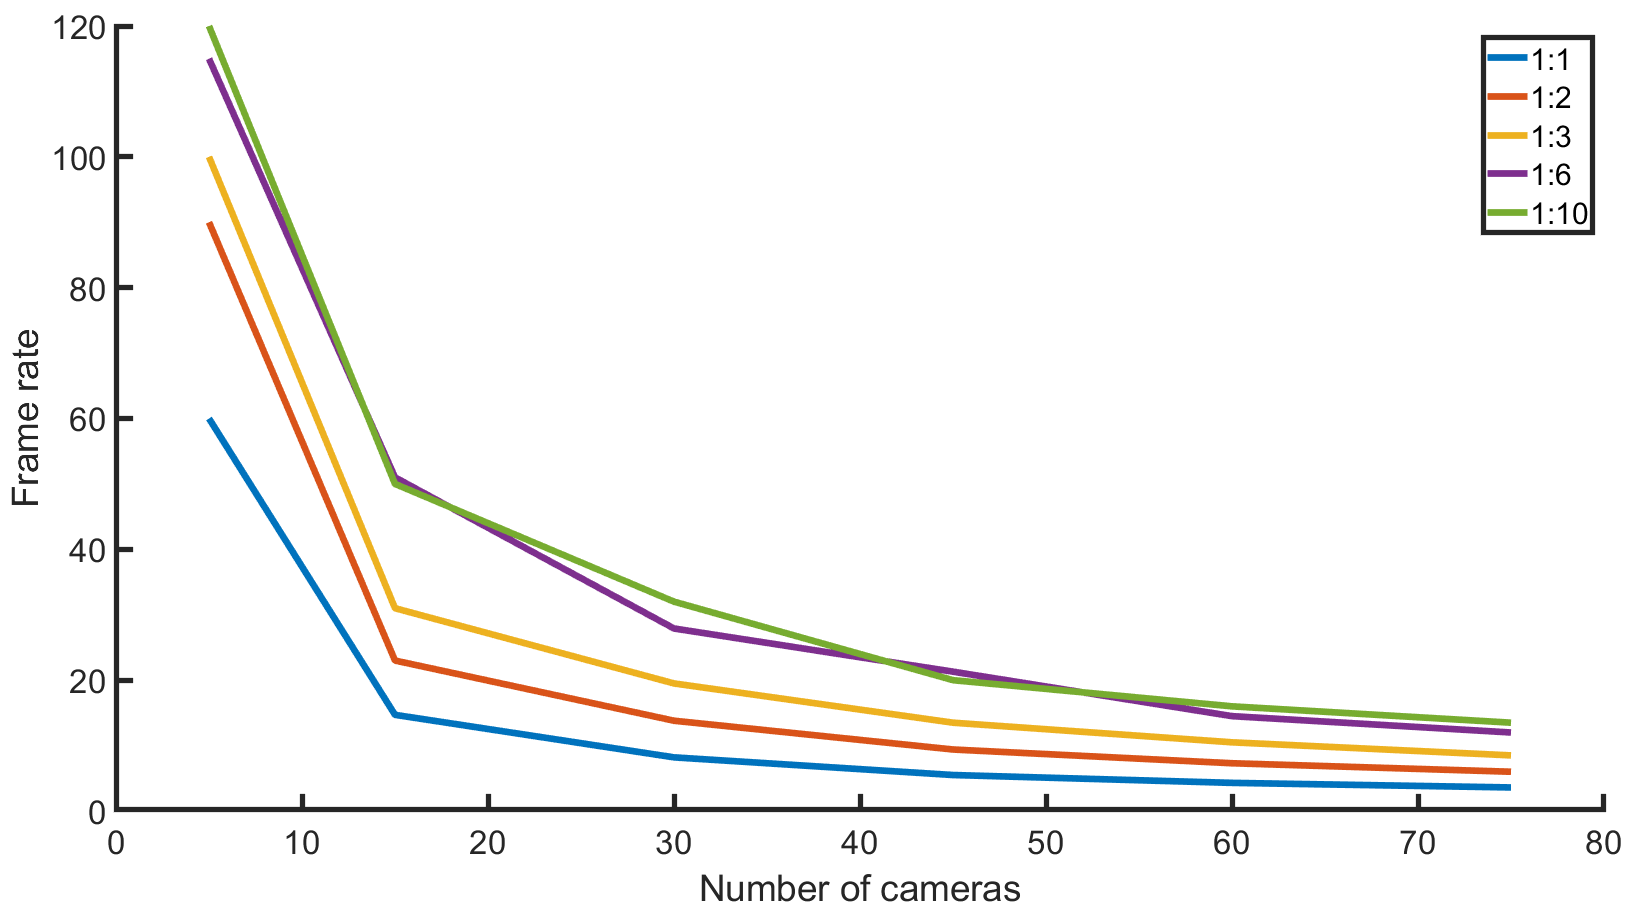
\includegraphics[width=0.7\textwidth]{06_Implementation/00_AirSim/Diagrams/frameRates.png}
    \caption{As the number of cameras are added to the scene the simulator frame rate decreases. By not rendering every camera on every frame the simulator frame rate increases. Each line represents a ratio for how often the camera renders, i.e. 1:2 means the camera frame is rendered every other game update.} \label{06:frameRates}
\end{wrapfigure}
The following changes aim to increase the output frame rate and optimise the APIs so that calls take less time, whilst trying to limit the impact on the simulator tick rate. 

When the vehicle starts, all attached cameras are loaded into a list. Instead of waiting for a request, the images are continually streamed to the server. This is illustrated in Figure~\ref{06:imageCaptureUpdated}. The user can enable and disable cameras to optimise the process. Every enabled camera stores the captured image in the server mapped to the vehicle and camera name. The figure shows how the API request does not have to interact directly with Unity, but can instead fetch the image directly from the server. This change means the server can request several hundred frames per second resulting in little delay between each API request. 

Figure~\ref{06:imageCaptureUpdated} makes it clear that an increased number of vehicles and cameras makes the update cycle slower. This means the game tick speed decreases. Figure~\ref{06:frameRates} shows the hyperbolic effect of how the game tick speed decreases with an increased number of cameras. It is important to note that the values are averages and could be impacted by other processes running simultaneously on the computer. The output frame rate will obviously decrease as well, but it will still match the game speed, so this does not matter. A way to counteract the increased number of cameras is not to render them on every game tick. The figure shows the average tick rate for the different ratios. A large ratio means that cameras are captured less often. This could be an issue if the vehicles were driving fast. It is also worth noting that a slow tick rate does not result in this issue. If the simulator tick rate is slow, and images are captured on every tick, the vehicle would only have moved a small amount as the simulation is running slowly. This means that compared to the simulator, the Python script can make a fast decision. It is also possible to deliberately decrease the tick speed if the processing in Python is slow. 

Overall, the outcome of this change is that there is a drastic increase in the framerate from the server. However, for a large number of cameras, the tick speed in Unity decreases. Future work could look at using UDP streaming to further increase the frame rate.  

\begin{figure}[p]
    \centering
    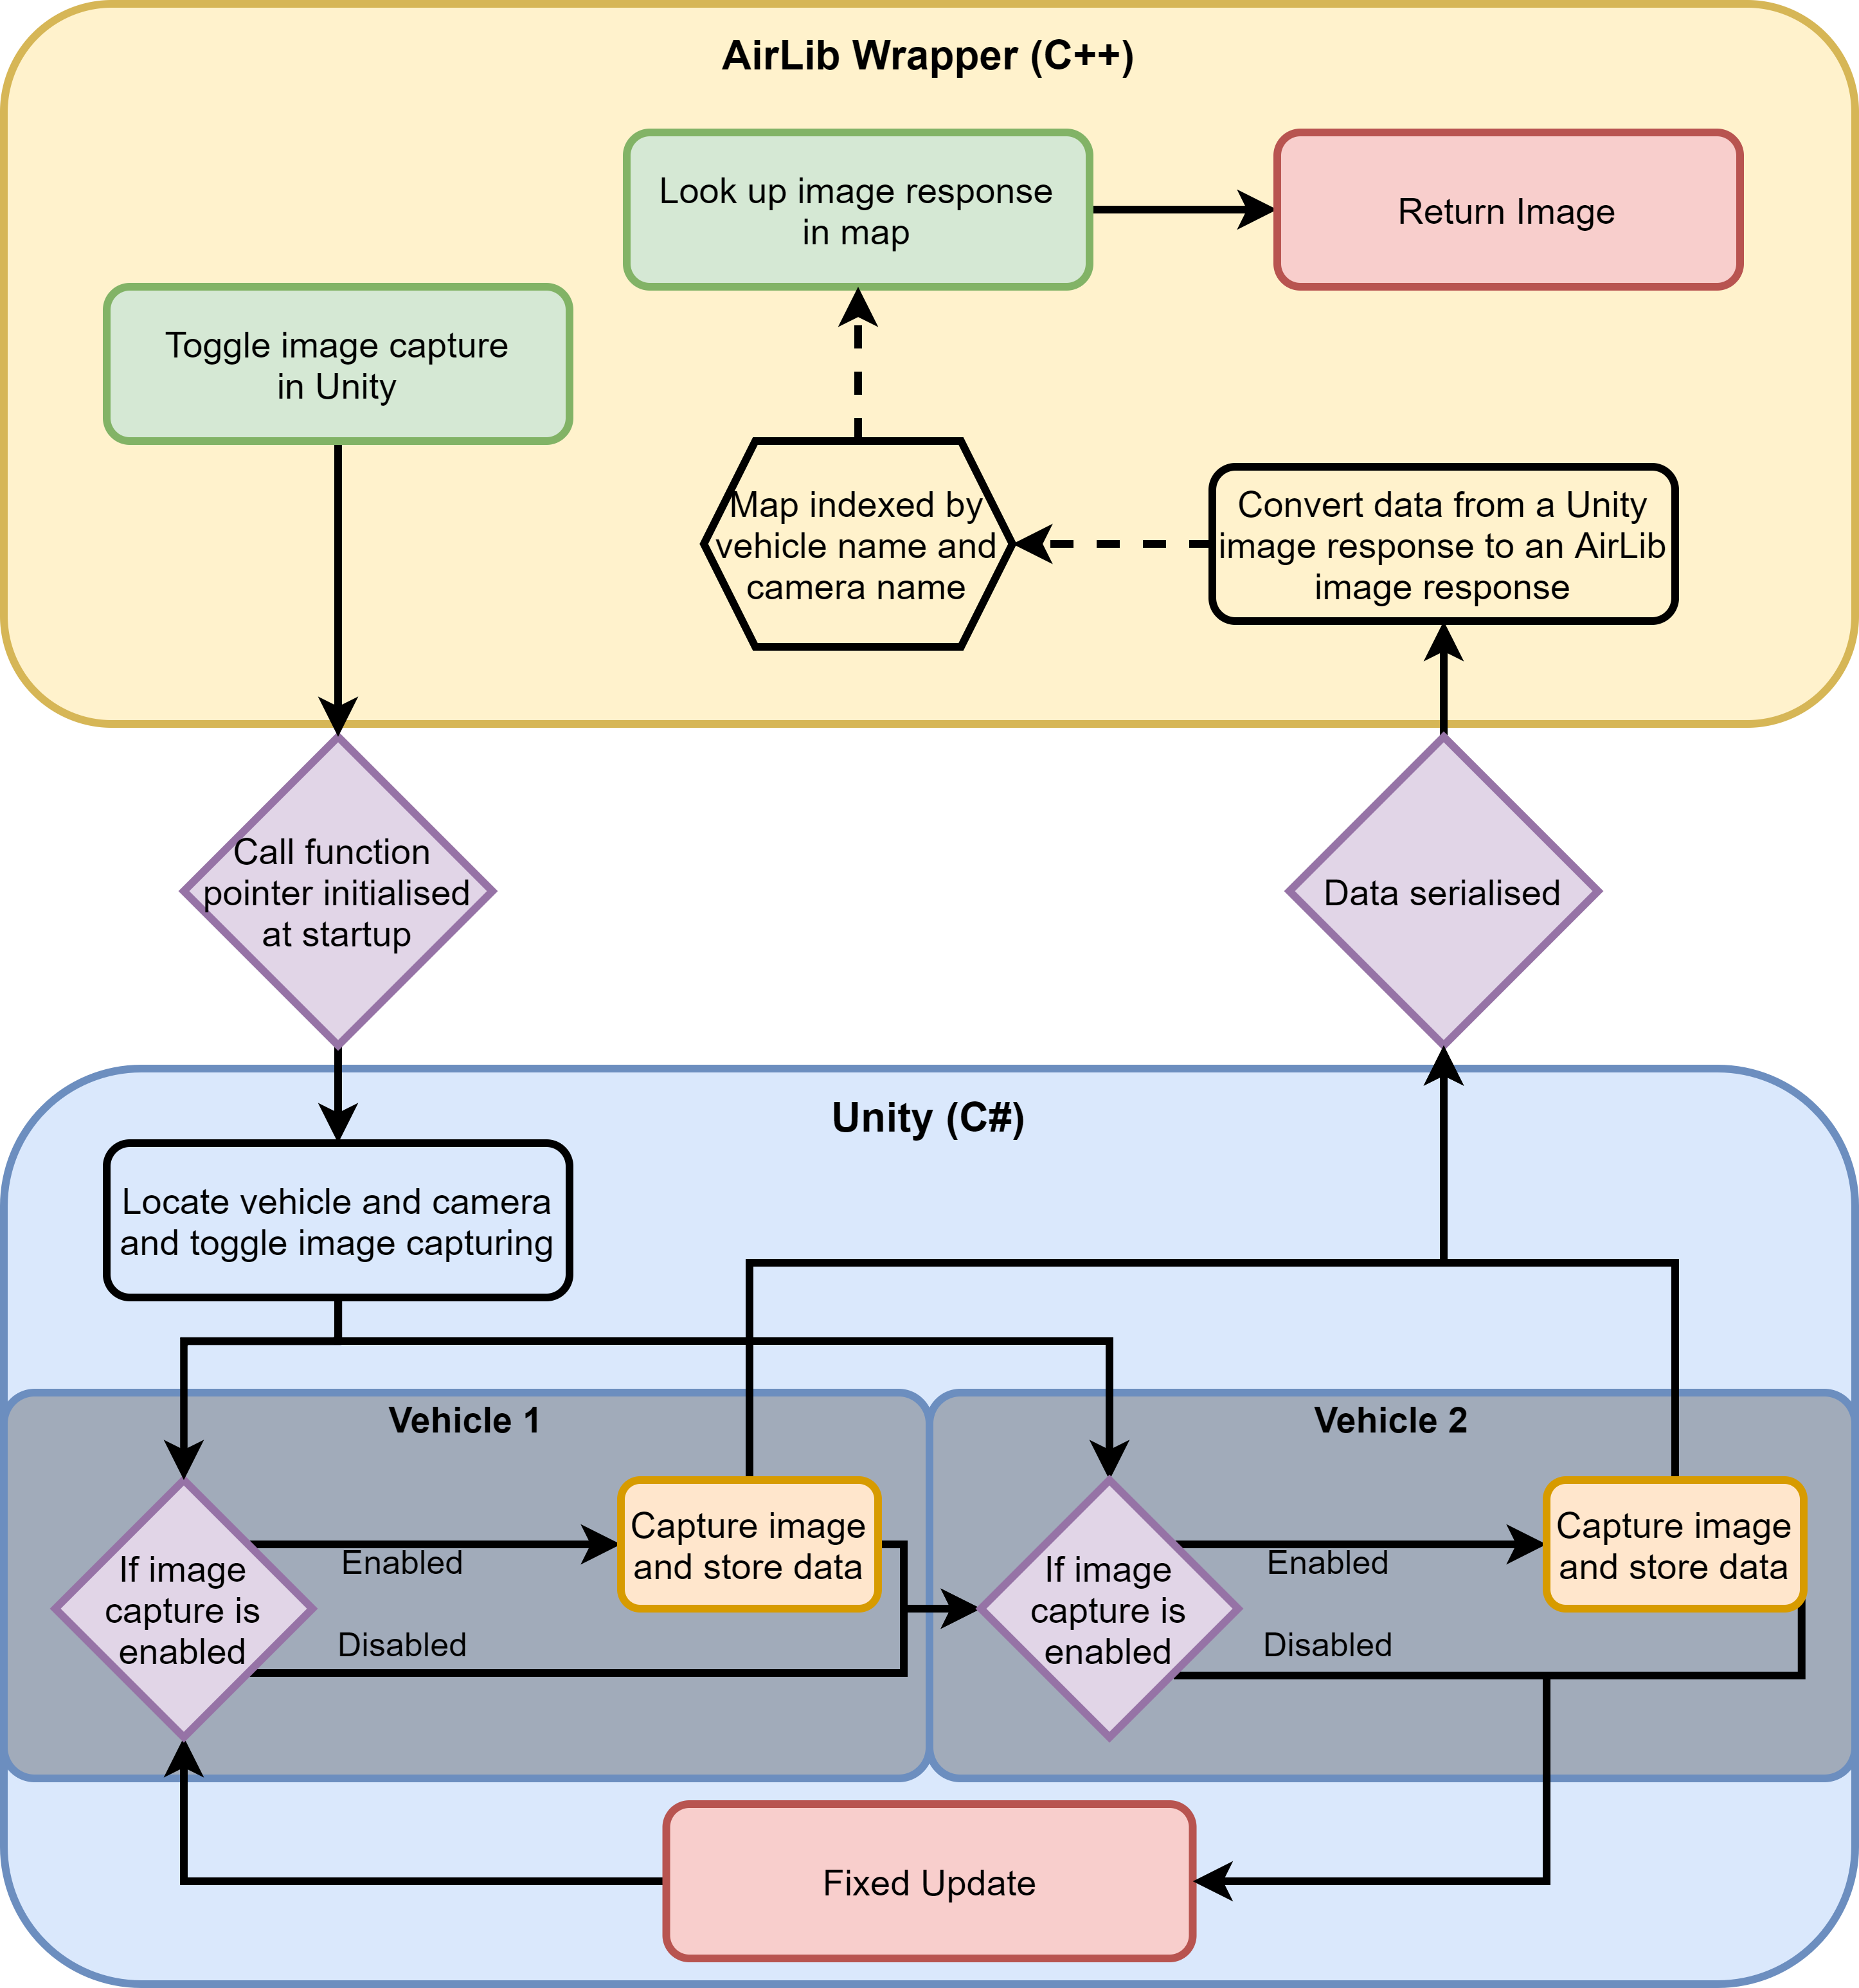
\includegraphics[width=1.0\textwidth]{06_Implementation/00_AirSim/Diagrams/imagecaptureUpdated.png}
    \caption{} \label{06:imageCaptureUpdated}
\end{figure}

\subsection{Adding Pedestrians}
This section will cover how pedestrians were added to the simulator. Pedestrians are one of the main forms of traffic wanted in this simulator. The pedestrians would be controllable through APIs in the same way as vehicles. 

The first step was to figure out how to create the pedestrians. The first option would be to use the standard Unity objects to create a character. This would be a simple capsule with a face. This would have been a bit simple for this project and having something more human-looking would be preferable. Another alternative was to download characters from mixamo\footnote{\url{ https://www.mixamo.com/}}. Mixamo is a technology company owned by Adobe which designs 3D characters and animation. The advantage of using Mixamo is that the characters come with a large range of animations as well as looking like humans. The disadvantage was having to download a large number of assets. Another way of creating character would be with the Unity character generation tool known as UMA2 (Unity Multipurpose Avatar). This allows for the character to have a variety of different shapes and attires. UMA can generate random models or they can be generated manually. Figure~\ref{} in the appendix shows some of the settings available. UMA  Figure~\ref{06:umaCharacters} shows some randomly generated characters inside Unity. These models will be used as the pedestrians. 

The next problem that had to be resolved was how to control the pedestrians. This was surprisingly simple. A character control script was already downloaded from the asset store when trying to use the Mixamo characters. Simply attaching this control script as well as the animation controller from the same asset made the characters run around. To make them walk, slowing down the direction speed worked. Another designed choice was made to have the controls for the pedestrians work similarly to the vehicles, i.e. pressing left and right would rotate the pedestrian rather than have it walk sideways on a grid. 

To make the pedestrians separated from the vehicles the server was divided into three components, the game server, pedestrian server and vehicle server. This was explained in the design chapter (Subsection~\ref{05:dividingServer}). Most of the basic APIs such as fetching available pedestrians, controlling the pedestrians and image capturing had to be reimplemented. These features were done similarly to how they work for the vehicles. The main difference being the struct with control commands being different. 

The next issue to be resolved was how to efficiently have UMA as a part of the project. UMA2 is over 500 MB and it would be unnecessary to have all of this pushed to GitHub. The solution was instead to have UMA as a requirement from the asset store. Prefabs were then created which would interact with the downloaded code. Script relating to AirSim would then be attached to these objects. 

Another small design decision that was made was how the cameras should behave. The animations make the pedestrians casually look around when standing still. To avoid this being an issue, the cameras are fixed facing forward from each eye. This means that the cameras are completely still when the pedestrians are walking. 

Overall the pedestrians took the most time to add to this project. Including dividing the server there was a lot of code that had to be changed throughout AirSim. One of the main challenges was that Unity does not display the error if there was an error caused by the AirLib DLL file. This made debugging the servers very difficult. Another issue that had to be resolved was that the original Unity version was too old to use all the UMA features. Updating Unity to a new version meant resolving other issues in AirSim and downloading outdated extensions. 
\begin{figure}[H]
    \centering
    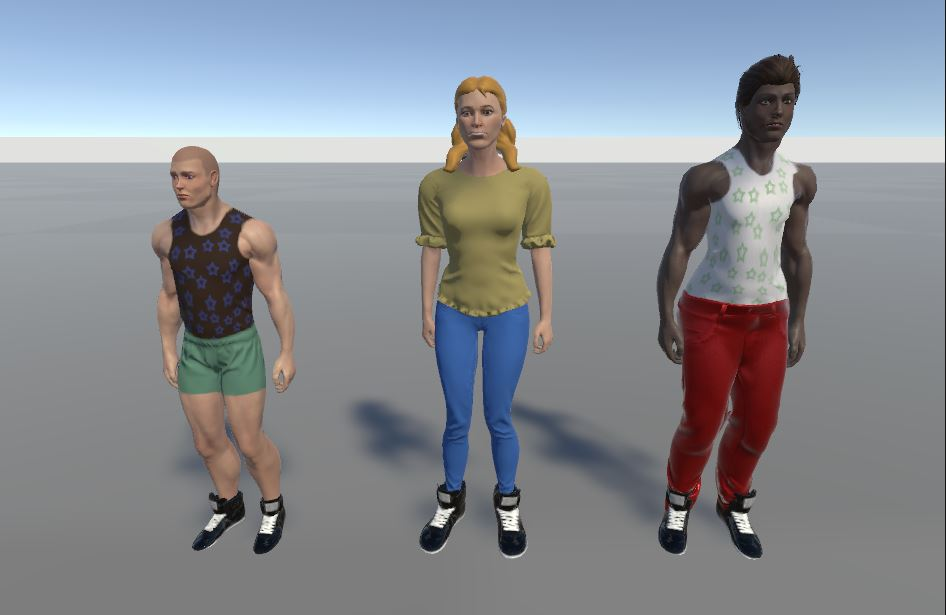
\includegraphics[width=0.6\textwidth]{06_Implementation/00_AirSim/Diagrams/RandomPedestrians.JPG}
    \caption{Randomly generated pedestrians using UMA2. UMA can be extended further by downloading additional assets which will add additional clothes, hair styles and more. UMA also allows for custom looking characters.} \label{06:umaCharacters}
\end{figure}

\subsection{Additional APIs}
This section will look at what additional APIs were added or modified.  It is worth noting that some of these features took a long time to add as they had to be done completely from scratch, whilst others could be done in less than an hour.

\subsubsection{Vehicle APIs}
\begin{enumerate}
    \item Updated \emph{enableAPIControls} - This is used to toggle the driving mode from through the API or manual inside the simulator.
    \item Updated \emph{simPrint} - Prints a debug statement from the vehicle.
    \item Added \emph{getVehicleTypes} - This returns a list of strings of the available vehicle types. This required significant changes to the simulator with roughly 15 files changed and 150 lines of code. The list of strings get converted into a char arrays with null terminated strings in C\# and then converted back into C++ strings in AirLib. Characters in C# are 16 bits, so every other character is skipped when reading the char array in C++.  This whole process was illustrated in Figure~\ref{05:stringList}. The commit with this can be found here\footnote{\url{https://github.com/tobhil98/MastersProject-AirSim/commit/22ab7c}}. A lot of time was spent trying to pass the arrays of strings from Unity to AirLib and then AirLib to Python.It is also worth nothing that this list could be extended with autonomous wheel chairs and other entities that would need the same controls and sensing abilities as a car. 
    \item Added \emph{simGetAllVehicles} - Returns a list of all vehicles in the scene. This is based off the getVehicleTypes API. 
    \item Updated \emph{setCarControls} - Updated how this was handled in Unity with several vehicles. Struct of car controls is passed from Python to Unity. 
    \item Updated \emph{getCarState} - Updated to handle several vehicles. Returns information about the car state such as speed, direction and location. 
    \item Added \emph{simGetLidar} - Added an API to fetch values form a Lidar beam. This is implemented in Unity using a ray cast to measure the distance to another object. Ideally this would be configurable in the request, but currently the beam is always from fixed points. 
    \item Updated \emph{simGetImages} - Fetches images using coroutines in Python. Decodes them and stores images in a dictionary indexed by the vehicle and camera name.
    \item Added \emph{simGetCameras} - Gets the names of the available cameras attached to the vehicle. 
\end{enumerate}

\subsubsection{Pedestrian APIs}
\begin{enumerate}
    \item Added \emph{ping} - Shows there is a connection with the pedestrian.
    \item Added \emph{reset} - Reset the pedestrian back to its original starting state.
    \item Added \emph{setPedestrianPose} - Sets the pedestrian position and rotation.
    \item Added \emph{getPedestrianPose} - Gets the pedestrian position and rotation.
    \item Added \emph{enableAPIControls} - This is based off the vehicles API. 
    \item Added \emph{simPrint} - Prints a debug statement from the pedestrian9.
    \item Added \emph{simGetAllPedestrians} - Returns a list of all pedestrians in the scene. This is based off the getVehicleTypes API. 
    \item Updated \emph{simGetImages} - Fetches images using coroutines in Python. Decodes them and stores images in a dictionary indexed by the vehicle and camera name.
    \item Added \emph{simGetCameras} - Gets the names of the available cameras attached to the pedestrian. 
\end{enumerate}


\subsubsection{Server APIs}
\begin{enumerate}
    \item Added \emph{ping} - Shows there is a connection with the server.
    \item Added \emph{getTickRate} - Fetches the current simulator tick rate in frames per second.
    \item Added \emph{simAddVehicle} - Explained in detail above how it is implemented. Spawns in a vehicle at a rotation at a specific location
    \item Added \emph{simAddPedestrian} - Spawns in a random pedestrian.
    \item Added \emph{simRemoveVehicle} - Removes the vehicle.    
    \item Added \emph{simRemovePedetrian} - Removes the pedestrian.
    \item Moved \emph{simPause} - APIs used to control the simulation speed. Moved from the old vehicle server.
    \item Moved \emph{simLogPrint} - Sends a debug print statement to Unity. 
\end{enumerate}


\subsection{Minor Features Added}
This section will briefly list other features added to the simulator. 
\begin{enumerate}
 \item \emph{Camera movement} - To be able to look around the simulator several different camera configurations have been implemented. These are to use in the simulator and cannot be controlled through APIs. One option is a free camera which allows the user to fly around the environment. The second option is to follow a specific entity. These options have been mapped to three number keys, key 1 for free movement, key 2 to follow vehicles and key 3 to follow pedestrians. When following vehicles or pedestrians the user can cycle through them by pressing tab (or shift+tab to cycle the other direction). The user can also easily move from following an entity to free camera movement by pressing the left shift key. 
 \item \emph{Rebuild script} - This is a simple update to the build script that compiles the AirLib dll. This change allows for faster compile time. This is very beneficial as it reduces the time to compile from over 10 minutes to just over 1 depending on the change made to the code. This change was a very small change to the build script which meant only files that had to be recompiled were recompiled, instead of rebuilding the whole project. 
 \item \emph{Upgraded Unity version} - The version Unity version used by AirSim by default is 2019.3.12, however there is a bug in this version which means internal projects cannot communicate with each other. The main issue here was that there was no way of communicating with the UMA code from the AirSim code. This was resolved by upgrading the version to 2019.3.13. This introduced a bunch of dependency issues as well as a couple of code issues that had to be fixed. This change should not impact future pull requests from the master repository as most features that are commonly used were backwards compatible. 
\end{enumerate}
%freecam and change between vehicles and entities
%Added global print from server - First thing to be added to get used to the codebase. 
%Rebuild script?
\subsection{Other Features Considered}
This section will briefly mention other features considered when adding features to Unity. The main reason for not adding these was in the interest of time.
\begin{enumerate}
\item \emph{Unity Navmesh}\footnote{\url{https://docs.unity3d.com/Manual/nav-CreateNavMeshAgent.html}} - This would allow pedestrians and vehicles to navigate around autonomously without needing to train a network. The navigation mesh can be laid on any surface to indicate where entities can go.
\item \emph{Unity Cloud Build}\footnote{\url{https://unity3d.com/unity/features/cloud-build}} - This is a framework that would allow testing the system online. However, this requires an advanced Unity license, so was not feasible for this project.
\end{enumerate}


\subsection{Extensibility}
The advantage of using AirSim and Unity is that the whole system is very flexible. As mention in the design chapter (Chapter~\ref{design}), AirSim allows for a variety of different languages to interact with the APIs. The whole project has made sure that future extensions should be simple to add if needed. This section will briefly look at how the existing features can help extend a future design.

\begin{enumerate}
\item \emph{Additional APIs} - This can be slightly complicated depending on the API. The API to base the new API off should be simGetImages. This is because it passes a struct of arguments to Unity, does some complex processing and passes a struct back. The struct has to be converted to different formats as it goes through AirSim as was shown in Figure~\ref{05:stringList}.
\item \emph{Additional Vehicle types} - This is done by adding the control script to the vehicle and then adding the prefab to the asset manager in the scene. To get all available vehicles for example the user could use the getVehicleTypes API which returns the names of the different types.  
\item \emph{Competly new type like wheelchairs} - This can either be added like an additional vehicle type with different physical properties. This would then have to use the same vehicle controls. It is also easy to look at how the pedestrian server works. Now the servers have been divided, creating more similar servers to how pedestrians were created is simple.  
\item \emph{Customise cameras} - Adding additional cameras to an object is done by creating a camera object onto the model and renaming the camera. The vehicle controller will find the object called Capture Cameras and iterate over the object to find all the cameras. The fetch available camera API listed above fetches all cameras attached to a specific object, so different vehicles can have a different number of cameras. 
\end{enumerate}

As AirLib works as a plugin to Unity, all Unity features are still available to use. This means adding something like VR or AR to the simulator should not be difficult if required.  

% Different vehicle designes by simply attaching the scritps
% Number of cameras
% Creating new types, for example autonomous chairs is simple by 




% Why did this not already exist
% •	Used to use config file. Not needed before.
% What changes had to be made
% •	Adding a new API to spawn vehicles, with position, rotation and name as arguments. 
% •	Server is connected to vehicle. Start server without vehicle
% How was the change made.
% •	Add APIs like diagram to spawn vehicles. 
% Challenges faced.
% •	Function pointers not bound by that point in time. Move vehicle spawning. 
% •	Issues with the threading

% Any limitations or known issues?

